\graphicspath{{fig/missing/}}

\chapter{Missing data}
\label{cha:missing}

Collecting data of flocking events is a demanding process. Along with the
technical challenges posed by data collection, flocking events are inherently
unpredictable, and so it is not possible to know when and where a flocking
event may occur next. In this way there can become a frustrating
`right-place-right-time' component to data collection.

Typically, recording equipment is set up in a fixed location where the
scientist believes a flocking event may occur. Stationary recording equipment
results in a fixed field of vision in which data may be captured.
Unfortunately, this stationary set-up can result in recording incomplete
flocking events. This may happen when flock members stray outside the field of
vision during a recording event. As the recording equipment is fixed in
location the field of vision cannot be adjusted to reinclude those who move
out-of-frame.

The flock members which move out of frame cannot be ignored during analysis:
although we may not observe their movements, they may still be influencing the
behaviour of the flock, and so must be accounted for. A simple but undesirable
solution is presented by the temptation to discard \emph{every} frame in which
any individual is out of view. This ``solution'' has the potential to
drastically reduce the amount of data available for analysis. As capturing
flocking events can be such an involved and time-consuming endeavour, it seems
remiss to discard observations and the information they contain.

In this chapter we will consider how we can handle flocking events which
contain missing observations. The movements of missing agents will not be
ignored, nor will data be discarded. Instead, we will work in a Bayesian framework
to adjust our posterior beliefs about model parameters to account for
unobserved behaviours. We will see that this can be achieved by integrating
over all the possible trajectories of missing agents. We show that
this approach gives more accurate results than the naive approach of discarding
data.

\section{Types of missingness}

When we consider flocking events with missing observations, it is important to
consider at which point during the sequence a given agent went missing. This is
because how we account for the missingness will depend on at which point during
the sequence the agent went missing.

Although there are many different circumstances which can result in an agent
leaving our visual field, here we shall inspect the two cases which we
consider as the most likely to occur. These two cases arise when agents are
out of frame at the \emph{beginning} of a recording event, or when
agents are out of frame at the \emph{end} of a recording event.

We shall integrate over the possible missing observations using a
Metropolis--Hastings scheme. A proposal mechanism for generating paths missing
at the beginning of a sequence is outlined. Proposed paths can then be accepted
or rejected using results from \cref{cha:sim_studies}. We will then show that
we can generate paths missing at the end of a sequence by implementing a Gibbs
sampler; sampling from our full conditional distributions to realise a
distribution of possible paths.

\subsection{Missing in the beginning}
\label{ssec:beg_missing}

We say that data is missing at the beginning of a flocking event if the
observer began recording the sequence before all agents had entered the frame.
When we consider this case we assume that all the flock members do eventually
enter the visual field, and so the total number of individuals in the flock is
known.

We imitate this set-up by forward simulating the Vicsek model and imposing a
fixed field of vision on top of the resulting data. We chose to forward
simulate $25$ agents for $40$ time steps. At time $t=1$ agents were directed
and positioned randomly within a square-cell of side length $L=1$. Agents
experienced noise generated from a generalised Student's $t$-distribution with
degrees of freedom $\nu=7$ and scale $\sigma_Y=0.075$. Each individual
interacted with neighbours positioned within distance $r=0.5$, and moved with
speed $v=0.03$.

The resulting simulated data is illustrated in \cref{subfig:beg_data}. The
rectangle overlain in black represents a fixed field of vision: analogous to
the fixed visual field generated by recording equipment in the field. The
movements of agents outside this fixed area are classified as missing and are
represented by the red trajectories. Agents move from the positions denoted by
the green markers, to the positions represented by the red makers. The ID
number of each agent, $i$, is shown at the beginning and end of its trajectory.
It can be seen that some agents were outside our visual field at the beginning
of the simulation. 

\cref{subfig:beg_missing} shows a schematic representing which data points of
our simulation were considered observed and which data points were classified
as missing. A blue gridpoint in location $(i, t)$ tells us that agent $i$
\emph{was observed} at time $t$. Conversely, a red maker at location $(i, t)$
indicates that agent $i$ \emph{was missing} at time $t$. From this schematic we
can see that a number of agents were classified as missing at time $t=1$: the
beginning of the simulation.

\begin{figure}[tbp]
  \captionsetup[subfigure]{oneside,
                           margin={0.7cm,0cm}}
  \begin{subfigure}[b]{0.5\textwidth}
    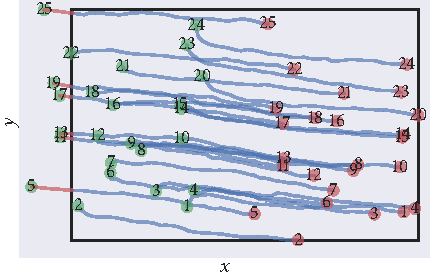
\includegraphics{beg/data.pdf}
    \caption{}
    \label{subfig:beg_data}
  \end{subfigure}%
  \begin{subfigure}[b]{0.5\textwidth}
    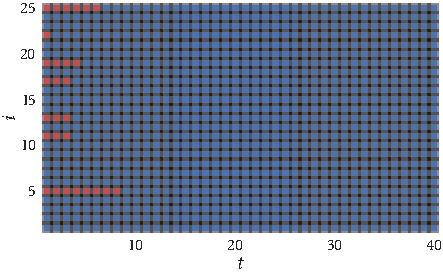
\includegraphics{beg/missing_array.pdf}
    \caption{}
    \label{subfig:beg_missing}
  \end{subfigure}
  \caption{Illustrating our forward simulation of the Vicsek model and the
    data considered missing. \subref{subfig:beg_data} Simulated trajectories.
    The rectangle overlain in black represents our imitation of a fixed
    field of vision: analogous to that of recording equipment used in the
    field. Agents travel from green marker to red marker, with their ID ($i$)
    shown at their start and end points. Data points outside of the rectangular
    region are classified as missing, and are shown by red trajectories.
    \subref{subfig:beg_missing} Summarising the missing and observed data
    points of our simulation. A blue gridpoint at location $(i, t)$ indicates
    that agent $i$ was within our visual field at time $t$. A red gridpoint at
    location $(i, t)$ indicates that agent $i$ was outside our visual field
    at time $t$.}
  \label{fig:beg_data}
\end{figure}

We may use \cref{eq:likelihood} to quantify the likelihood of observing a
flock's movements. However, to compute the likelihood we must observe the
positions and directions of each individual in every frame. With this, to
evaluate the likelihood of a flock with missing observations we must propose
candidate values for the missing data points. To do so we shall work backwards
from our first observation of each missing agent.

We propose missing directions of motion backwards in time from our first
observation of each missing agent. A symmetric proposal distribution is used
to propose a missing direction $\theta_{i,t-1}$ as:
\begin{equation}
  \label{eq:propose_beg_dir}
  \theta_{i,t-1}^{\star} \given  \theta_{i,t}, \nu, \sigma_Y
    \sim t_{\nu}(\theta_{i,t}, \sigma_Y),
\end{equation}
where $t_{\nu}$ denotes a generalised Student's $t$-distribution with $\nu$
degrees of freedom. An alternative proposal scheme could be formulated using
the interaction term $\angmean{\theta}_{i,t}$ as:
\begin{equation}
  \label{eq:propose_beg_dir_alt}
  \theta_{i,t-1}^{\star} \given \angmean{\theta}_{i,t}, \nu, \sigma_Y
    \sim t_{\nu}(\angmean{\theta}_{i,t}, \sigma_Y).
\end{equation}
However, this proposal mechanism is more computationally expensive than the
proposal scheme outlined in \cref{eq:propose_beg_dir}, as it necessitates the
computation of $\angmean{\theta}_{i,t}$. For highly aligned flocks we expect
\cref{eq:propose_beg_dir,eq:propose_beg_dir_alt} to propose similar candidate
values, with \cref{eq:propose_beg_dir} doing so at a smaller computational
expense. It is for this reason that we shall use the proposal distribution of
\cref{eq:propose_beg_dir}.

Having worked backwards in time to propose plausible values for the unobserved
directions of motion, we can now use these values to realise the corresponding
proposed paths. To do so we rearrange \cref{eq:positional_update} to see:
\begin{equation}
  \label{eq:step_back}
  \bm{x}_{i,t} = \bm{x}_{i,t+1} - \bm{v}_{i,t}.
\end{equation}
Recall from \cref{sec:vicsek_model} that $\bm{v}_{i,t}$ is constructed to have
direction $\theta_{i,t+1}$ and speed $v$. Given $\theta_{i,t+1}$, we may
compute $\bm{v}_{i,t} = (\cos\theta_{i,t+1}, \sin\theta_{i,t+1})^Tv$. With
this, and reindexing $t\mapsto t-1$, we may rewrite \cref{eq:step_back} as:
\begin{equation}
  \label{eq:propose_beg_pos}
  \bm{x}_{i,t-1} = \bm{x}_{i,t} - (\cos\theta_{i,t}, \sin\theta_{i,t})^Tv.
\end{equation}

Having proposed candidate values for the missing directions of motions with
\cref{eq:propose_beg_dir}, we can use \cref{eq:propose_beg_pos} to compute the
proposed paths which these directions correspond to. As these proposed
paths represent missing data, if any of the proposed positions lie
\emph{within} our frame of vision, then we must reject these proposals and
continue onto the next iteration of our scheme.

Having values for the positions and directions of motion of every individual at
every time step, we may use \cref{eq:likelihood} to quantify the likelihood of
these paths, given some model parameters.

To infer the Vicsek model's parameters from our simulated data we shall
implement a random walk Metropolis--Hastings sampler. At each iteration of the
sampler we shall propose model parameters and candidate values for the missing
observations. These proposed data points are then accepted or rejected along
with the proposed model parameters, with probability given by the acceptance
probability. With this, each missing observation introduces an additional
dimension to the posterior distribution, and so increases complexity. As a
result, if the amount of missing data increases then the computational demand
of the problem increases.

We simulate our random-walk sampler for $10^5$ iterations, and thin the
resulting output by a factor of $10$. The output is thinned to reduce the
autocorrelation between successive samples. We assess convergence by inspecting
trace plots of the simulated chains. \cref{fig:beg_dir_trace} visualises the
chains targeting the directions of motion $\theta_{6,4}$, $\theta_{6,3}$,
$\theta_{6,2}$ and $\theta_{6,1}$, which were classified as missing. From this
plot we see well-behaved chains oscillating regularly around a fixed location,
evidencing convergence. The true values of the missing observations are
indicated by the horizontal green lines. See that the true values are all
captured within the oscillations of our chains, but that the further back in
time we work the greater the oscillations become. The magnitude of the
oscillations increase as we extrapolate further backwards in time and become
more uncertain about the possible movements of missing agents.

\begin{figure}[tbp]
  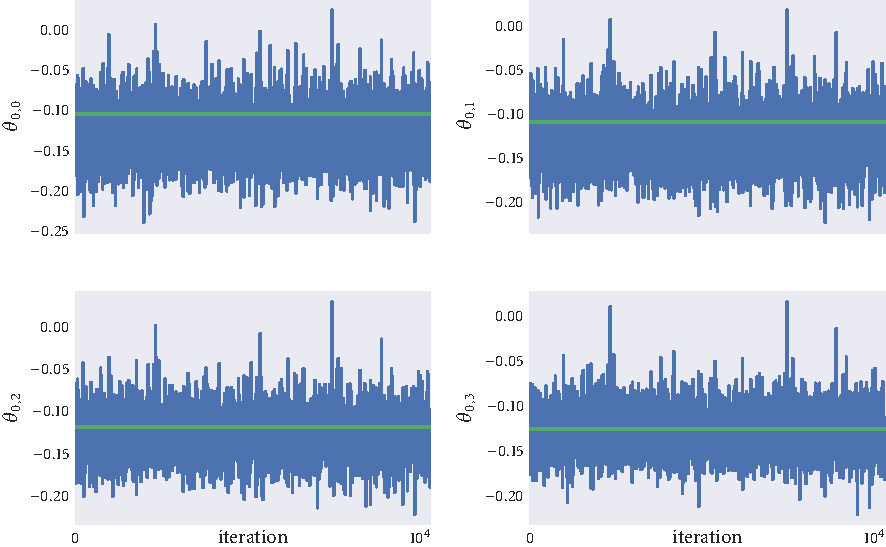
\includegraphics{beg/dir_trace.pdf}
  \caption{Chains targeting directions of motion missing at the beginning of a
  simulation. Each trajectory was simulated for $10^6$ iterations. To reduce
  the autocorrelation between samples the output was thinned by a factor of
  $100$. The true values of the missing directions are shown by the horizontal
  green lines. The true values are captured within our posterior densities.}
  \label{fig:beg_dir_trace}
\end{figure}

\cref{fig:beg_x_trace} shows chains targeting the missing $x$ co-ordinates of
agent $6$ over frames $4$, $3$, $2$ and $1$. The chains targeting the $x$
co-ordinates are related to the chains targeting the missing directions through
\cref{eq:propose_beg_pos}. We see further evidence that our chains have
converged, and that the further back in time we work the less certain we become.

\begin{figure}[tbp]
  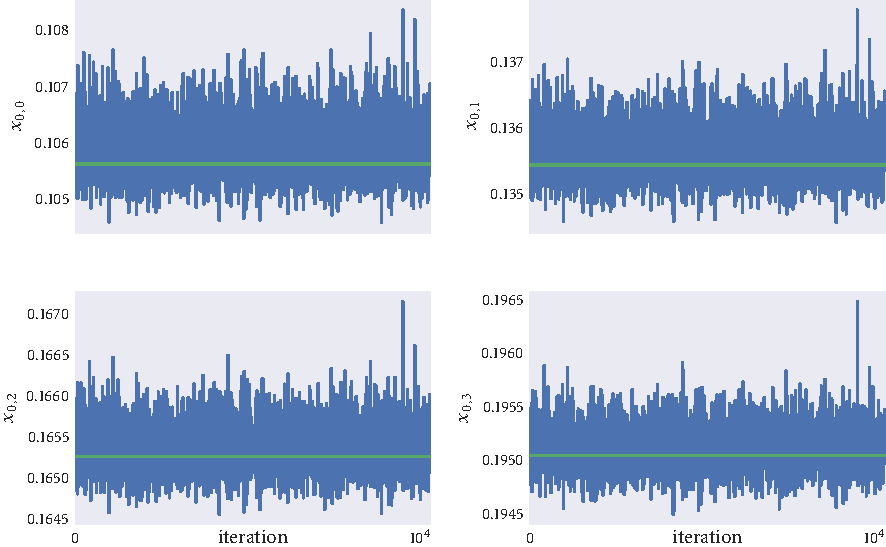
\includegraphics{beg/x_trace.pdf}
  \caption{Trajectories of the $x$ co-ordinates of agents corresponding to the
  directions of motion seen in \cref{fig:beg_dir_trace}. Sampled directions of
  motion are related to sampled co-ordinates through \cref{eq:propose_beg_pos}.
  The true missing $x$ co-ordinates are overlain in green and lie within the
  posterior density.}
  \label{fig:beg_x_trace}
\end{figure}

As with the hierarchical models considered in \cref{sec:hier_mod_studies}, we
now have a posterior distribution with a large number of dimensions, and so
assessing and presenting every posterior density becomes impractical. Instead,
we summarise the output of our chains targeting the missing observations in
\cref{fig:beg_summary}. Each panel of \cref{fig:beg_summary} shows box and
whisker plots summarising our posterior samples. The yellow markers show the
posterior median, the inner-extent of the whiskers show the upper and lower
quartiles, and the outer-extent of the whiskers show the posterior median
$\pm1.5\times\text{IQR}$.

\begin{figure}[tbp]
  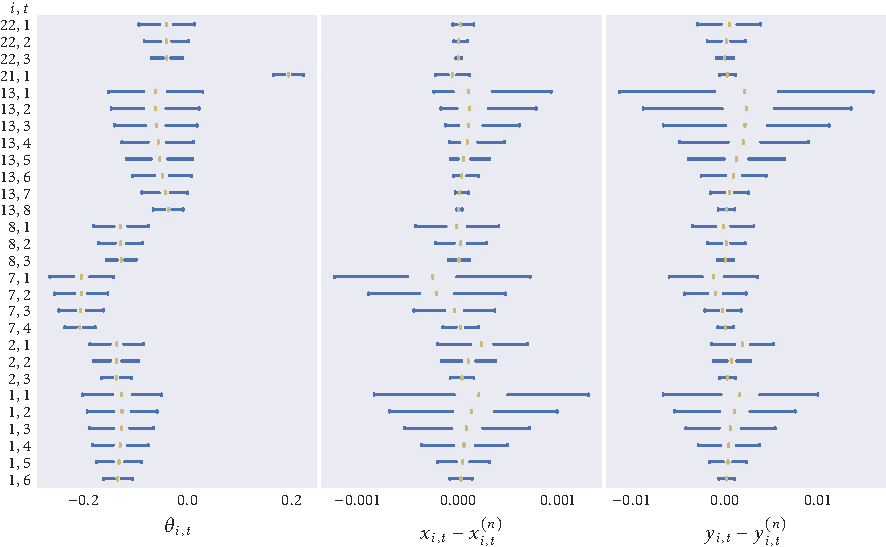
\includegraphics{beg/summary.pdf}
  \caption{Summarising the posterior samples targeting the missing directions
  of motion (left), $x$ co-ordinates (centre), and $y$ co-ordinates (right).
  True values are shown by the green markers, and posterior medians are shown
  by the yellow markers. The box and whisker plots show the upper and lower
  quartiles as well as the median $\pm1.5\times\text{IQR}$. Realisations of the
  missing positions are subtracted from the corresponding true values to make
  comparison easier.}
  \label{fig:beg_summary}
\end{figure}

The left-most panel of \cref{fig:beg_summary} summarises the posterior
densities representing our beliefs about the missing directions of motion. The
green markers represent true values. See that as we extrapolate further back in
time our posterior variance increases, as we would expect. The $x$ and $y$
co-ordinates corresponding to these directions are shown in the central and
right-most panels. As the between-agent variance in positions is much greater
than our posterior variances, to compare all the inferred positions in one plot
we first subtract the samples from the true values. This results in box and
whisker plots centered approximately around zero (shown by the green markers):
indicating that our posterior beliefs accurately captured the true values.
Again, we see that our posterior variance about the inferred positions
increases the further back in time we extrapolate.

We have shown that we can capture missing observations by implementing a
Metropolis--Hastings sampler. Now that we have this, we wish to inspect how
having missing observations has effected our parameter uncertainty. We also
wish to investigate how our approach to missing data compares to the more
naive approach of discarding frames which don't capture every individual. To
make this comparison we re-perform parameter inference on the simulated data,
in the first instance increasing our field of vision to capture all
agents, and in the second instance discarding frames where any individual is
missing. We expect that the posterior variance about the model parameters with
the missingness accounted for should be greater than or equal to the posterior
variance had there been no missingness. Similarly, had we discarded the frames
with missingness, we would expect a posterior variance greater than or equal to
the posterior variance with the missingness integrated over. 

\cref{fig:beg_compare} compares posterior densities of the model parameters
under three different regimes: the flocking event without any missingness
(blue), the event with the missingness integrated out (red), and the event with
the missingness discarded (purple). From this plot we see that integrating over
the missing observations provides very similar posterior densities to if we had
observed all the data. We see that our approach to handling missingness gives
smaller posterior variance than the naive approach of discarding observations,
indicating the efficacy of our approach. As the computational demand of the
problem increases as more data goes missing, effort should still be made by the
scientist to minimise the total amount of missingness incurred during data
collection.

\begin{figure}[tbp]
  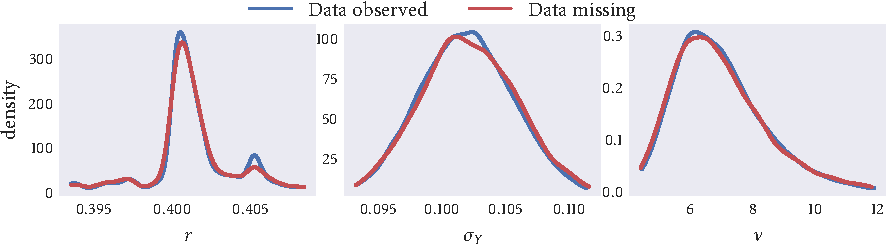
\includegraphics{beg/compare_params.pdf}
  \caption{Comparing posterior beliefs about the Vicsek model parameters had
    all the data been observed (blue); with the missingness integrated out
    (red), and when discarding frames which any individual is missing from
    (purple). The posterior densities are shown by kernel density estimates
    of the posterior samples.}
  \label{fig:beg_compare}
\end{figure}

\subsection{Missing in the end}
\label{ssec:end_missing}

We say that data is missing at the end of a flocking event if some individuals
leave the frame of vision before the recording event was completed. When we
consider this case we assume that agents which leave the frame do not later
re-enter. We imitate this set-up by simulating the movements of $25$
individuals over $40$ frames, according to the specifications of the Vicsek
model (parameters $r=0.45$, $\sigma_Y=0.07$ and $\nu=7$), and overlaying a fixed
field of vision. The resulting data is visualised in \cref{fig:end_data}.

\begin{figure}[tbp]
  \captionsetup[subfigure]{oneside,
                           margin={0.7cm,0cm}}
  \begin{subfigure}[b]{0.5\textwidth}
    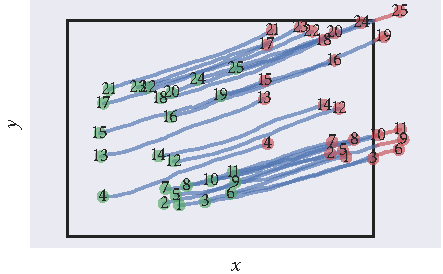
\includegraphics{end/data.pdf}
    \caption{}
    \label{subfig:end_data}
  \end{subfigure}%
  \begin{subfigure}[b]{0.5\textwidth}
    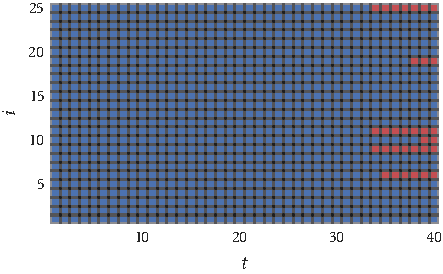
\includegraphics{end/missing_array.pdf}
    \caption{}
    \label{subfig:end_missing}
  \end{subfigure}
  \caption{Individuals missing at the end of a sequence.
  \subref{subfig:end_data} Twenty-five agents are simulated for forty frames
  according to the rules of the Vicsek model. Agents travel from the positions
  denoted by the green markers to those denoted by the red markers. The ID of
  each agent is shown at its start and end point. A fixed field of vision is
  emulated by the rectangle overlain in black. Any movements which occur
  outside this area are classified as missing; shown by trajectories
  transitioning from blue to red.
  \subref{subfig:end_missing} A representation of which data points of our
  simulation were observed and which were classified as missing. A blue tile at
  location $(i, t)$ indicates that agent $i$ was within our field of vision at
  time $t$. Conversely, a red tile at location $(i, t)$ indicates that agent
  $i$ was outside our field of vision---that is, missing---at time $t$.}
  \label{fig:end_data}
\end{figure}

To fit one of our models to this data we must be able to evaluate the
likelihood as specified in \cref{eq:likelihood}. This likelihood involves a
product over $i=1,\ldots,N$ and $t=1,\ldots,T$, and so we must have data to
represent these observations. As some agents are out of frame at the end of the
sequence, we do not have all the observations necessary to evaluate the
likelihood.

We can propose trajectories for the missing agents by forward simulating the
model from each agent's last observed position. As we are able to write down
our full conditional distributions about future directions of motion
(\cref{eq:students_update}) this step becomes akin to performing a Gibbs step.
With this there is no accept / reject step for the sampled trajectories, and so
new missing paths are evaluated at every iteration of our sampler. As the
sampled trajectories represent missing observations, any samples that are
generated within our field of vision are discarded and new trajectories are
sampled instead. This Gibbs step is embedded within a Metropolis--Hastings
sampler which works to infer the model parameters of the Vicsek model.

\cref{fig:end_dir_trace} shows the chains targeting the missing directions of
motion of agent $i=6$. These trajectories show evidence of convergence and are
seen to capture the true values of the missing data (green). These directions
are related to the $y$ component of the missing positions (shown in
\cref{fig:end_y_trace}) via \cref{eq:positional_update}, and again capture the
true values of the missing data.

In \cref{fig:end_dir_trace,fig:end_y_trace} we only inspect a small amount of
the total missingness targeted by our inference. \cref{fig:end_summary}
summarises our posterior beliefs about all the missing observations of our
simulated data. We see that in all cases the true values (green) are captured
within our posterior densities (blue). From the central and rightmost panels of
\cref{fig:end_summary} we see that posterior variance (uncertainty) increases
the further into the future we extrapolate.

\begin{figure}[tbp]
  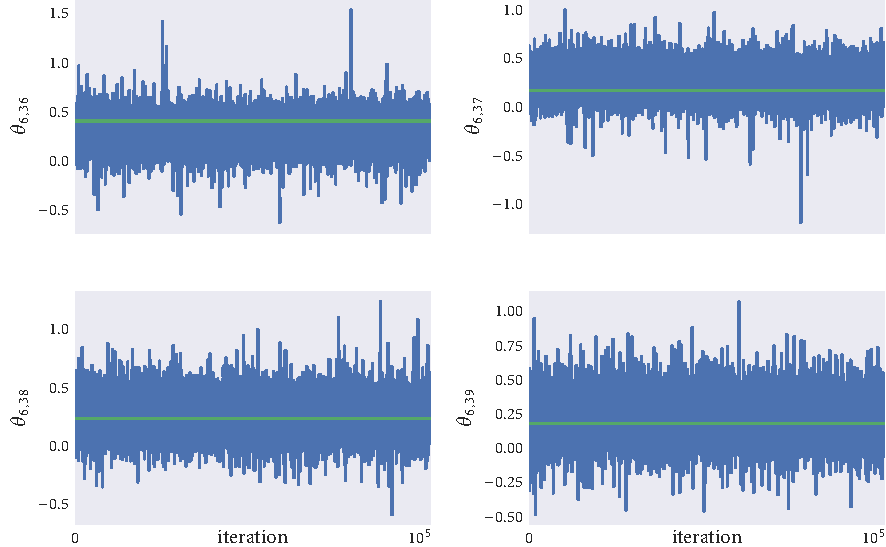
\includegraphics{end/dir_trace.pdf}
  \caption{Trace plots targeting directions of motion missing at the end of the
  simulated flocking event. The chains give strong evidence of convergence and
  show that the true values of the missing directions (green) are captured within
  our posterior densities.}
  \label{fig:end_dir_trace}
\end{figure}
\begin{figure}[tbp]
  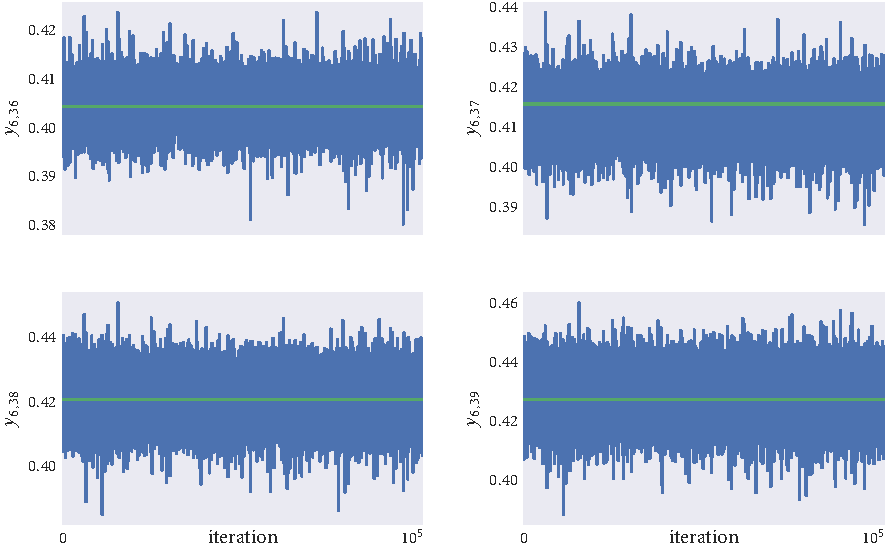
\includegraphics{end/y_trace.pdf}
  \caption{Trajectories targeting the $y$ component of the missing positions of
    agent $i=6$. The chains show evidence of convergence: oscillating around
    a fixed point with constant variance. The true values (green) are
    captured within the oscillations of the chains.}
  \label{fig:end_y_trace}
\end{figure}
\begin{figure}[tbp]
  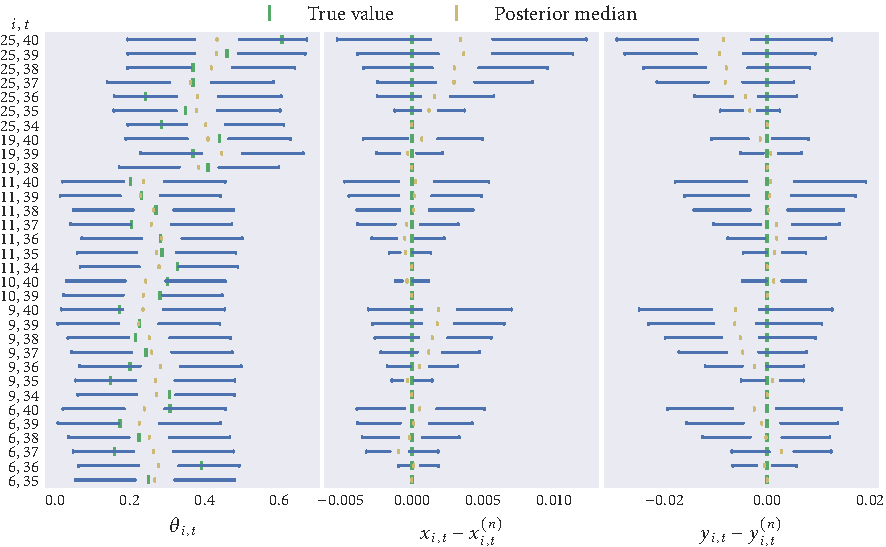
\includegraphics{end/summary.pdf}
  \caption{Summarising the posterior densities of the missing directions (left
  panel), $x$ co-ordinates (central panel), and $y$ co-ordinates (right
  panel). For comparative ease the samples of the missing positions are
  subtracted from the true missing positions. The true values being
  targeted are shown by the green markers, and all lie within the box and
  whisker plots representing our posterior densities. As we extrapolate further
  into the future we see that our posterior variance increases, as our
  uncertainty about the values of the missing observations increases.}
  \label{fig:end_summary}
\end{figure}

\cref{fig:end_summary} shows that our approach to missingness is able to
capture data missing at the end of a recording event. We now wish to inspect
how this approach has effected our posterior beliefs. To do so we perform
parameter inference on the simulated data as if all the data had been contained
within our field of vision. In addition to this we perform the same inference
but discarding all the frames in which any agent was out of view. The model
parameters inferred under these three scenarios are compared in
\cref{fig:end_compare}. We see that integrating out the missingness reveals
results similar to as if we had observed all the data, and that the naive
approach of discarding missingness resulted in a larger posterior variance.

The Gibbs sampler explores the sample space more efficiently than the
Metropolis--Hastings algorithm, an artefact of Gibbs' lack of an accept / reject
step. As a result we can handle data missing at the end of a sequence with
less computational expense than data missing at the beginning of a sequence.
We conclude that although all effort should be made by the scientist to avoid
recording sequences with any missing observations, where possible care should
be taken to bias the occurrence of data missing at the end of a sequence over
data missing at the beginning of a sequence.

\begin{figure}
  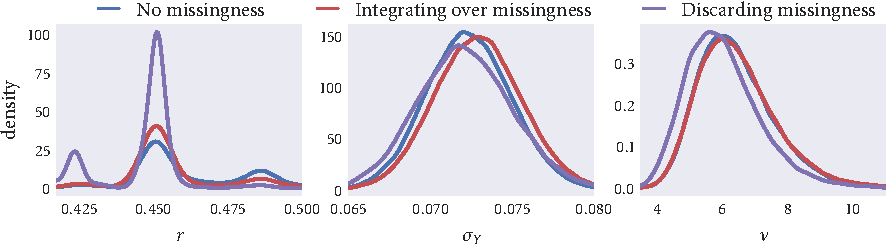
\includegraphics{end/compare_params.pdf}
  \caption{Kernel density estimates of the model parameters inferred from
  simulated data. The blue kernels represent posterior densities when the
  field of vision was widened to include all movements; the red kernels
  show posterior densities when the missingness was integrated out, and the
  purple kernels represent the posterior samples when all the frames
  containing missing data were discarded.}
  \label{fig:end_compare}
\end{figure}

\subsection{Missing in the beginning and end}

Having demonstrated that we can handle sequences with observations missing at
the beginning of a sequence and sequences with observations missing at the end
of a sequence, we now seek to verify that we can handle sequences with data
missing at the beginning \emph{and} end. Having considered these two cases
separately we now consider them jointly. 

To handle sequences with data missing at the beginning and end, it is
sufficient to use the Gibbs step as outlined in \cref{ssec:end_missing} to
sample paths missing at the end of the sequence, and the Metropolis--Hastings
algorithm to propose paths missing at the beginning of the sequence, as in
\cref{ssec:beg_missing}.
